\chapter{Geometric Calculus - Integration}
\section{Line Integrals}
If $\fof{F}{x}$ is a multivector field and $\fof{x}{\lambda}$ is a parametric representation of
a vector path (curve) then the line Integral of $F$ along the path $x$ is defined to be
\be
\int\fof{F}{x}\deriv{x}{\lambda}d\lambda = \int F\: dx \equiv \lim_{n\mapsto\infty} \sum_{i=1}^{n}\bar{F}^{i}\Delta x^{i}
\ee
where
\be
\begin{array}{cc}
\Delta x^{i} = x_{i}-x_{i-1}, & \bar{F}^{i} = \half\paren{\fof{F}{x_{i-1}}+\fof{F}{x_{i}}}
\end{array}
\ee
if $x_{n}=x_{1}$ the path is closed.  Since $dx$ is a vector, that is
$\fof{F}{x}\deriv{x}{\lambda} \ne \deriv{x}{\lambda}\fof{F}{x}$, a more general line integral would be
\be
\int\fof{F}{x}\deriv{x}{\lambda}\fof{G}{x}\;d\lambda = \int\fof{F}{x}dx\:\fof{G}{x} 
\ee
The most general form of line integral would be
\be
\int \fof{\mathsf{L}}{\partial_{\lambda}x;x}\:d\lambda = \int \fof{\mathsf{L}}{dx}
\ee
where $\fof{\mathsf{L}}{a}=\fof{\mathsf{L}}{a;x}=$ is a multivector-valued linear function of $a$. The
position dependence in $\mathsf{L}$ can often be suppressed to streamline the notation.
\section{Surface Integrals}
The next step is a directed surface integral. Let $\fof{F}{x}$ be a multivector field and let a surface
be parametrized by two coordinates $\fof{x}{x^{1},x^{2}}$.  Then we can define a directed surface measure by
\be
dX = \pdiff{x}{x^{1}}\w\pdiff{x}{x^{2}}\: dx^{1}dx^{2} = \eb_{1}\w\eb_{2}\; dx^{1}dx^{2}
\ee
A directed surface integral takes the form
\be
\int F\:dX = \int F \eb_{1}\w\eb_{2}\: dx^{1}dx^{2}
\ee
In order to construct some of the more important proof it is necessary to express the surface integral
as the limit of a sum. This requires the concept of a triangulated surface as shown
\begin{figure}[htbp]
\begin{center}
\scalebox{0.4}{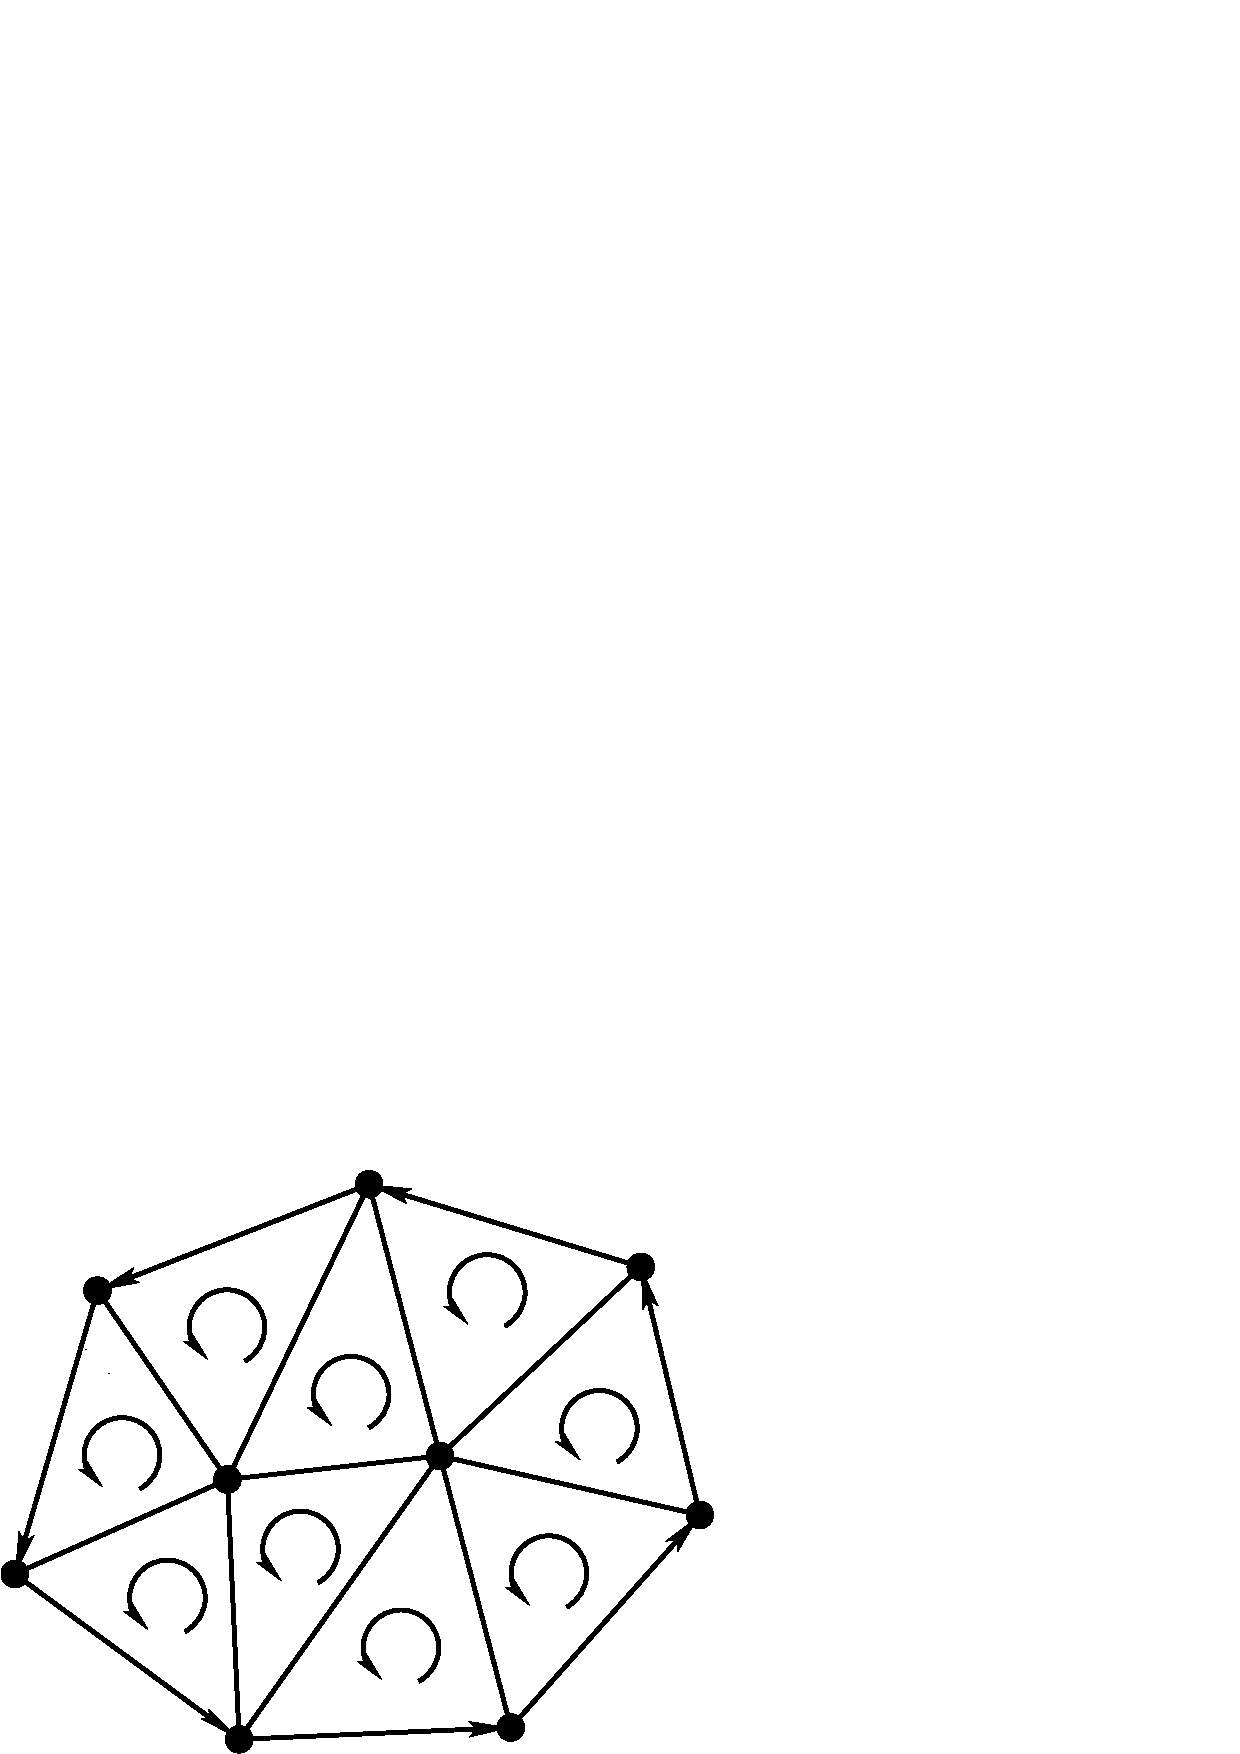
\includegraphics{simplex.png}}
\caption{Triangulated Surface}
\end{center}
\end{figure}
Each triangle in the surface is described by a planar simplex as shown
\begin{figure}[htbp]
\begin{center}
\scalebox{0.5}{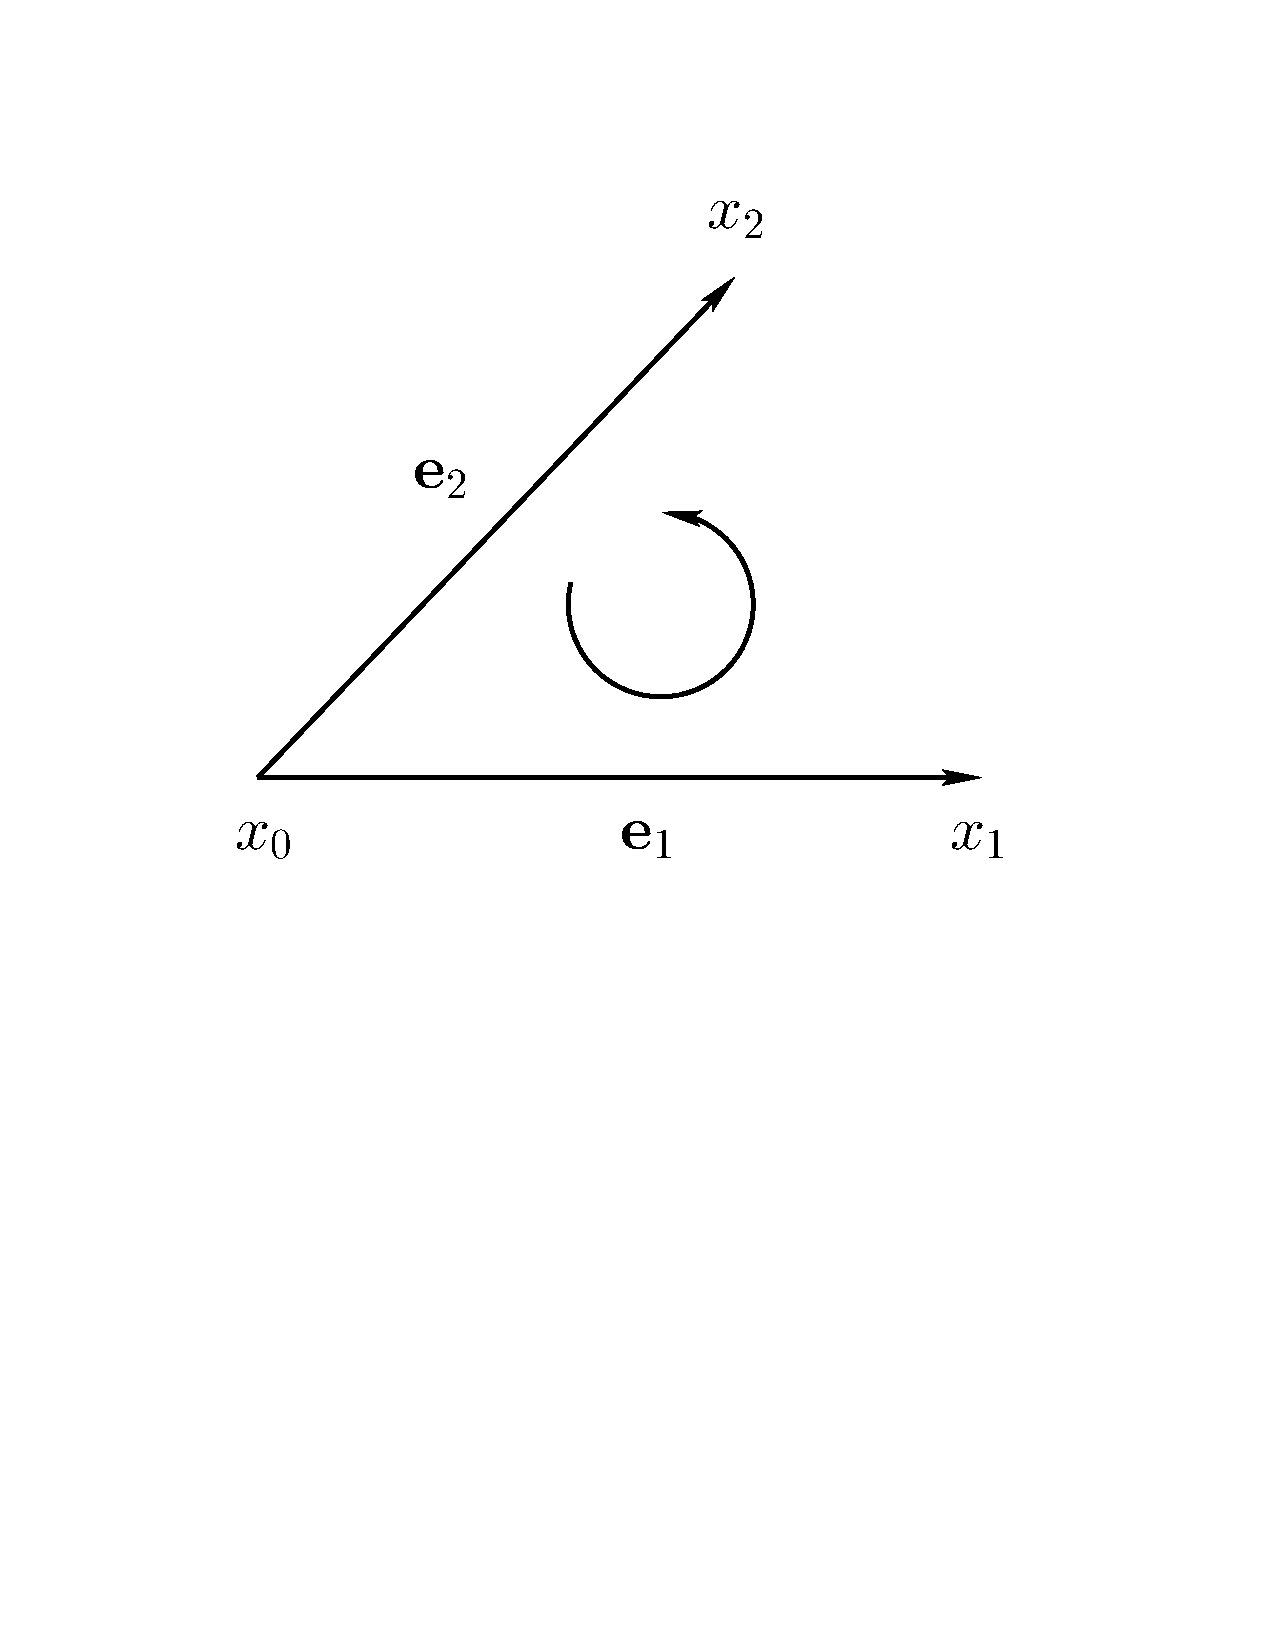
\includegraphics{planarsimplex.png}}
\caption{Planar Simplex}
\end{center}
\end{figure}
The three vertices of the planar simplex are $x_{0}$, $x_{1}$, and $x_{2}$ with the vectors
$\eb_{1}$ and $\eb_{2}$ defined by
\be
\begin{array}{cc}
\eb_{1} = x_{1}-x_{0}, & \eb_{2} = x_{2}-x_{0}
\end{array}
\ee
so that the surface measure of the simplex is
\be
\Delta X \equiv \half\eb_{1}\w\eb_{2} = \half\paren{x_{1}\w x_{2}+x_{2}\w x_{0}+x_{0}\w x_{1}}
\ee
with this definition of $\Delta X$ we have
\be
\int F\: dX  \equiv \lim_{n\mapsto\infty} \sum_{k=1}^{n} \bar{F}^{k}\Delta X^{k} 
\ee
where $\bar{F}^{k}$ is the average of $F$ over the $k^{th}$ simplex.
\section{Directed Integration - $n$-dimensional Surfaces}

\subsection{$k$-Simplex Definition}

In geometry, a simplex or $k$-simplex is an $k$-dimensional analogue of a triangle. Specifically, a simplex is the 
convex hull of a set of $(k + 1)$ affinely independent points in some Euclidean space of dimension $k$ or higher.

For example, a 0-simplex is a point, a 1-simplex is a line segment, a 2-simplex is a triangle, a 3-simplex is a 
tetrahedron, and a 4-simplex is a pentachoron (in each case including the interior).
A regular simplex is a simplex that is also a regular polytope. A regular $k$-simplex may be constructed from a regular 
$(k-1)$-simplex by connecting a new vertex to all original vertices by the common edge length.

\subsection{$k$-Chain Definition (Algebraic Topology)}

A finite set of $k$-simplexes embedded in an open subset of $\Re^{n}$ is called an affine $k$-chain. The simplexes in a
chain need not be unique, they may occur with multiplicity. Rather than using standard set notation to denote an affine 
chain, the standard practice to use plus signs to separate each member in the set. If some of the simplexes
have the opposite orientation, these are prefixed by a minus sign. If some of the simplexes occur in the set more than once,
these are prefixed with an integer count. Thus, an affine chain takes the symbolic form of a sum with integer coefficients.

\subsection{Simplex Notation}

If $\paren{x_{0},x_{1},\dots,x_{k}}$ is the $k$-simplex defined by the $k+1$ points 
$x_{0},x_{1},\dots,x_{k}$.  This is abbreviated by
\be
\chn{x}{k} = \paren{x_{0},x_{1},\dots,x_{k}}
\ee 
The order of the points is important for a simplex, since it specifies the orientation of the simplex.  If any two
adjacent points are swapped the simplex orientation changes sign.  The boundary operator for the simplex is denoted by $\partial$
and defined by
\be\label{eq211}
\partial\chn{x}{k} \equiv \sum_{i=0}^{k} \paren{-1}^{i}\chn{x_{0},\dots,\breve{x}_{i},\dots,x_{k}}{k-1}
\ee
To see that this make sense consider a triangle $\chn{x}{3} = \paren{x_{0},x_{1},x_{2}}$. Then
\begin{align}
\partial\chn{x}{3} &= \chn{x_{1},x_{2}}{2}-\chn{x_{0},x_{2}}{2}+\chn{x_{0},x_{1}}{2} \nonumber \\
                   &= \chn{x_{1},x_{2}}{2}+\chn{x_{2},x_{0}}{2}+\chn{x_{0},x_{1}}{2}
\end{align}
each 2-simplex in the boundary 2-chain connects head to tail with the same sign.

Now consider the boundary of the boundary
\begin{align}
\partial^{2}\chn{x}{3} &= \partial\chn{x_{1},x_{2}}{2}+\partial\chn{x_{2},x_{0}}{2}+\partial\chn{x_{0},x_{1}}{2}
                                \nonumber \\
                       &= \chn{x_{1}}{1}-\chn{x_{2}}{1}+\chn{x_{2}}{1}-\chn{x_{0}}{1}+\chn{x_{0}}{1}
                                 -\chn{x_{1}}{1} \nonumber \\
                       &= 0
\end{align}
We need to prove is that in general $\partial^{2}\chn{x}{k}=0$. To do this consider the boundary of the $i^{th}$
term on thr r.h.s. of equation~\ref{eq211} letting 
$\Aijk{ij}{k-2}= \chn{x_{0},\dots,\breve{x}_{i},\dots,\breve{x}_{j},\dots,x_{k}}{k-1}$. 

Then
\be\label{eq214}
\begin{array}{l}
\hspace{-0.25in}\partial\chn{x_{0},\dots,\breve{x}_{i},\dots,x_{k}}{k-1} = \\ 
 \hspace{0.2in}\left \{\begin{array}{cc}
 i = 0: & {\ds \sum_{j=1}^{k}\paren{-1}^{j-1}\Aijk{ij}{k-2} } \\
 0<i<k: & {\ds \sum_{j=0}^{i-1}\paren{-1}^{j}\Aijk{ij}{k-2}+\sum_{j=i+1}^{k}\paren{-1}^{j-1}\Aijk{ij}{k-2} } \\
 i = k: & {\ds \sum_{j=0}^{k-1}\paren{-1}^{j}\Aijk{ij}{k-2} }
\end{array}\right \}
\end{array} 
\ee
The critical point in equation~\ref{eq214} is that the exponent of $-1$ in the second term on the r.h.s. is
not $j$, but $j-1$.  The reason for this is that when $x_{i}$ was removed from the simplex the vertices were
{\bf not} renumbered.  We can now express the boundary of the boundary in terms of the following matrix elements
($\Bijk{ij}{k-2} = \paren{-1}^{i+j}\Aijk{ij}{k-2}$) as
\begin{align}\label{eq248}
\partial^{2}\chn{x}{k} = & \sum_{j=1}^{k}\paren{-1}^{j-1}\Aijk{0j}{k-2}+\paren{-1}^{k}\sum_{j=0}^{k-1}\paren{-1}^{j}\Aijk{kj}{k-2} \nonumber \\
                         & +\sum_{i=1}^{k-1}\paren{-1}^{i}\left(\sum_{j=0}^{i-1}\paren{-1}^{j}\Aijk{ij}{k-2}
                            +\sum_{j=i+1}^{k}\paren{-1}^{j-1}\Aijk{ij}{k-2} \right) \nonumber \\
                       = & -\sum_{j=1}^{k}\Bijk{0j}{k-2}+\sum_{j=0}^{k-1}\Bijk{kj}{k-2} \nonumber \\ 
                       & +\sum_{i=1}^{k-1}\sum_{j=0}^{i-1}\Bijk{ij}{k-2}-\sum_{i=1}^{k-1}\sum_{j=i+1}^{k}\Bijk{ij}{k-2} = 0
\end{align}
The consider $\Bijk{ij}{k-2}$ as a matrix ($i$-row index, $j$-column index). The matrix is symmetrical and in equation~\ref{eq248} you
are subtracting all the elements above the main diagonal from the elements below the main diagonal so that $\partial^{2}\chn{x}{k} = 0$ and
the boundary of a boundary of a simplex is zero.

Now add geometry to the simplex by defining the vectors
\be
\begin{array}{cc}
e_{i} = x_{i}-x_{0}, & i=1,\dots,k,
\end{array}
\ee
and the directed volume element
\be\label{eq196}
\Delta X = \bfrac{1}{k!}e_{1}\w\cdots\w e_{k}
\ee
We now wish to prove that
\be
\int_{\smplx{x}{k}} dX = \Delta X
\ee
Any point in the simplex can be written in terms of the coordinates $\ldi{i}$ as
\be\label{eq237}
x = x_{0}+\sum_{i=1}^{k} \ldi{i}e_{i}
\ee
with restrictions
\be
\begin{array}{ccc}
0\le\ldi{i}\le 1 & \mbox{and} & {\ds\sum_{i=1}^{k}\ldi{i} \le 1}
\end{array}
\ee
First we show that
\be
\int_{\smplx{x}{k}} dX = \int_{\smplx{x}{k}} e_{1}\w\cdots\w e_{k}\: \dldi{1}\cdots\dldi{k} = \Delta X
\ee
or
\be
\int_{\smplx{x}{k}} \dldi{1}\cdots\dldi{k} = \bfrac{1}{k!}
\ee
define $\Ldi{j}=1-\sum_{i=1}^{j}\ldi{i}$ (Note that $\Ldi{0}=1$). From the restrictions on the $\ldi{i}$'s we have
\be\label{eq201}
\int_{\smplx{x}{k}} \dldi{1}\cdots\dldi{k} = \int_{0}^{\Ldi{0}}\dldi{1}\int_{0}^{\Ldi{1}}\dldi{2}\cdots
	\int_{0}^{\Ldi{k-1}}\dldi{k}
\ee
To prove that the r.h.s of equation~\ref{eq201} is $1/k!$ we form the following sequence and use induction
to prove that $V_{j}$ is the result of the first $j$ partial Integrations of equation~\ref{eq201}
\be
V_{j} = \bfrac{1}{j!}\paren{\Ldi{k-j}}^{j}
\ee
Then
\begin{align}
V_{j+1} &= \int_{0}^{\Ldi{k-j-1}} \dldi{k-j}V_{j} \nonumber \\
		&= \int_{0}^{\Ldi{k-j-1}} \dldi{k-j}\bfrac{1}{j!}\paren{\Ldi{k-j-1}-\ldi{k-j}}^{j}
			\nonumber \\
        &= \bfrac{-1}{\paren{j+1}j!}\left[\paren{\Ldi{k-j-1}-\ldi{k-j}}^{j+1}
            \right]_{0}^{\Ldi{k-j-1}} \nonumber \\
        &=  \bfrac{1}{\paren{j+1}!}\paren{\Ldi{k-j-1}}^{j+1}\label{eq243}
\end{align}
so that $V_{k} = 1/k!$ and the assertion is proved.
Now let there be a multivector field $\fof{F}{x}$ that assumes the values $F_{i} = \fof{F}{x_{i}}$ at the vertices
of the simplex and define the interpolating function
\be\label{eq244}
\fof{f}{x} = F_{0}+\sum_{i=1}^{k}\ldi{i}\paren{F_{i}-F_{0}}
\ee
We now wish to show that
\be\label{eq205}
\int_{\smplx{x}{k}}f\: dX = \bfrac{1}{k+1}\paren{\sum_{i=0}^{k}F_{i}}\Delta X = \bar{F}\: \Delta X
\ee
To prove this we must show that
\be\label{eq206}
\int_{\smplx{x}{k}}\ldi{i}\: dX = \bfrac{1}{k+1} \Delta X,\quad \forall\:\ldi{i}
\ee
To do this consider the integral (equation~\ref{eq243} with $V_{j}$ replaced by $\ldi{k-j}V_{j}$) 
\begin{align}
\int_{0}^{\Ldi{k-j-1}}\dldi{k-j}\:\ldi{k-j}V_{j} &= \int_{0}^{\Ldi{k-j-1}}
		\dldi{k-j}\bfrac{1}{j!}\ldi{k-j}\paren{\Ldi{k-j-1}-\ldi{k-j}}^{j} \nonumber \\
	&= \bfrac{1}{\paren{j+2}!}\paren{\Ldi{k-j-1}}^{j+2}
\end{align}
Note that since the extra $\ldi{i}$ factor occurs in exactly one of the subintegrals for each different $\ldi{i}$ the
final result of the total integral is multiplied by a factor of $\frac{1}{\paren{k+1}}$ since the weight of the total integral 
is now $\frac{1}{\paren{k+1}!}$ and the assertion (equation~\ref{eq206} and hence equation~\ref{eq205}) is proved.

Now summing over all the simplices making up the directed volume gives
\be\label{eq208}
\int_{\mbox{volume}} F\: dX = \lim_{n\mapsto\infty} \sum_{i=1}^{n}\bar{F}^{i} \Delta X^{i}
\ee
The most general statement of equation~\ref{eq208} is
\be
\int_{\mbox{volume}} \fof{\mathsf{L}}{dX} = \lim_{n\mapsto\infty} \sum_{i=1}^{n}\fof{\bar{\mathsf{L}}^{i}}{\Delta X^{i}}
\ee
where $\fof{\mathsf{L}}{F_{n};x}$ is a position dependent linear function of a grade-$n$ multivector $F_{n}$ and 
$\bar{\mathsf{L}}^{i}$ is the average value of $\fof{\mathsf{L}}{dX}$ over the vertices of each simplex.

An example of this would be
\be
	\fof{\mathsf{L}}{F_{n};x} = \fof{G}{x} F_{n} \fof{H}{x} 
\ee
where $\fof{G}{x}$ and $\fof{H}{x}$ are multivector functions of $x$.
\section{Fundamental Theorem of Geometric Calculus}
Now prove that the directed measure of a simplex boundary is zero 
\be\label{eq218}
\Delta\paren{\partial\chn{x}{k}} = \Delta\paren{\partial\chn{x_{0},\dots,x_{k}}{k}} = 0
\ee
Start with a planar simplex of three points
\be
\partial\chn{x_{0},x_{1},x_{2}}{2} = \chn{x_{1},x_{2}}{1}-\chn{x_{0},x_{2}}{1}+\chn{x_{0},x_{1}}{1}
\ee
so that
\be
\Delta\paren{\partial\chn{x_{0},x_{1},x_{2}}{2}} = \paren{x_{2}-x_{1}}-\paren{x_{2}-x_{0}}+\paren{x_{1}-x_{0}} = 0
\ee
We shall now prove equation~\ref{eq218} via induction.  First note that
\be
\Delta\chn{\breve{x}_{i}}{k-1} = \left\lbrace
\begin{array}{cc}
i = 0: & \bfrac{1}{k-1}\Delta\chn{\breve{x}_{0}}{k-2}\w\paren{x_{k}-x_{1}} \\
0 < i \le k-1: & \bfrac{1}{k-1}\Delta\chn{\breve{x}_{i}}{k-2}\w\paren{x_{k}-x_{0}}
\end{array}
 \right\rbrace 
\ee
and
\be
\Delta\chn{\breve{x}_{k}}{k-1} = \bfrac{1}{\paren{k-1}!}\paren{x_{1}-x_{0}}\W\cdots\W\paren{x_{k-1}-x_{0}}
\ee
so that
\be
\Delta\paren{\partial\chn{x}{k}} = 
   \bfrac{1}{k-1}\sum_{i=1}^{k-1}\paren{-1}^{i}\Delta\chn{\breve{x}_{i}}{k-2}\w\paren{x_{k}-x_{0}}+\mathcal{C} \nonumber \\
\ee
where
\be
\mathcal{C} = \bfrac{1}{k-1}\Delta\chn{\breve{x}_{0}}{k-2}\w\paren{x_{k}-x_{1}}
+\paren{-1}^{k}\Delta\chn{\breve{x}_{k}}{k-1}
\ee
if we let $\delta = x_{0}-x_{1}$ we can write
\be
\mathcal{C} = \bfrac{1}{k-1}\Delta\chn{\breve{x}_{0}}{k-2}\w\paren{x_{k}-x_{0}}+
               \bfrac{1}{k-1}\Delta\chn{\breve{x}_{0}}{k-2}\w\delta
              +\paren{-1}^{k}\Delta\chn{\breve{x}_{k}}{k-1}
\ee
Then
\begin{align}
\Delta\chn{\breve{x}_{0}}{k-2}\w\delta &= \bfrac{1}{\paren{k-2}!}\paren{x_{2}-x_{1}}\W\cdots\W\paren{x_{k-1}-x_{1}}\W\delta \\
                                       &= \bfrac{1}{\paren{k-2}!}\paren{x_{2}-x_{0}+\delta}\W\cdots\W\paren{x_{k-1}-x_{0}+\delta}\W\delta \\
                                       &= \bfrac{1}{\paren{k-2}!}\paren{x_{2}-x_{0}}\W\cdots\W\paren{x_{k-1}-x_{0}}\W\delta \\
                                       &= \bfrac{\paren{-1}^{k-2}}{\paren{k-2}!}\delta\W\paren{x_{2}-x_{0}}\W\cdots\W\paren{x_{k-1}-x_{0}} \\                                                                    									   &= \bfrac{\paren{-1}^{k-1}}{\paren{k-2}!}\paren{x_{1}-x_{0}}\W\paren{x_{2}-x_{0}}\W\cdots\W\paren{x_{k-1}-x_{0}}
\end{align}
Thus
\begin{align}
\bfrac{-1}{k-1}\Delta\chn{\breve{x}_{0}}{k-2}\w\delta &= \\
                                                      &\hspace{-1.5in}= \bfrac{\paren{-1}^{k}}{\paren{k-1}!}\paren{x_{1}-x_{0}}\W\paren{x_{2}-x_{0}}\W\cdots\W\paren{x_{k-1}-x_{0}} \\
                                                      &\hspace{-1.5in}= \paren{-1}^{k}\Delta\chn{\breve{x}_{k}}{k-1}
\end{align}
However
\be
\paren{-1}^{k}\Delta\chn{\breve{x}_{k}}{k-1} = \bfrac{-1}{k-1}\Delta\chn{\breve{x}_{0}}{k-2}\w\delta
\ee
so that
\be\label{eq226}
\mathcal{C} = \bfrac{1}{k-1}\Delta\chn{\breve{x}_{0}}{k-2}\w\paren{x_{k}-x_{0}}
\ee
and
\begin{align}
\Delta\paren{\partial\chn{x}{k}} &=\bfrac{1}{k-1}\paren{\sum_{i=0}^{k-1}\paren{-1}^{i}\Delta\chn{\breve{x}_{i}}{k-2}}
                                   \w\paren{x_{k}-x_{0}} \nonumber \\
                                 &= \bfrac{1}{k-1}\paren{\Delta\paren{\partial\chn{x}{k-1}}}
                                     \w\paren{x_{k}-x_{0}} \nonumber \\
                                 &= 0
\end{align}
We have proved equation~\ref{eq218}.  Note that to reduce equation~\ref{eq226} we had to use that for any set of vectors $\delta,y_{1},\dots,y_{k}$ we have
\be\label{eq228}
\delta\w\paren{y_{1}+\delta}\w\cdots\w\paren{y_{k}+\delta} = \delta\w y_{1}\w\cdots\w y_{k}
\ee
Think about equation~\ref{eq228}. It's easy to prove ($\delta\W \delta = 0$)!

Equation~\ref{eq218} is sufficient to prove that the directed integral over the surface of simplex is
zero
\be
\oint_{\partial\chn{x}{k}}dS = \sum_{i=0}^{k}\paren{-1}^{i}\int_{\chn{\breve{x}_{i}}{k-1}}
                                              \hspace{-0.5in}dX = \Delta\paren{\partial\chn{x}{k}} = 0
\ee
The characteristics of a general volume are:
\begin{enumerate}
\item A general volume is built up from a chain of simplices.
\item Simplices in the chain are defined so that at any common boundary the directed
 areas of the bounding faces are equal and opposite.
\item Surface integrals over two simplices cancel over their common face.
\item The surface integral over the boundary of the volume can be replaced by the sum
of the surface integrals over each simplex in the chain.
\end{enumerate}
If the boundary of the volume is closed we have
\be\label{eq230}
\oint dS = \lim_{n\mapsto\infty}\sum_{a=1}^{n}\oint dS^{a} = 0 
\ee
Where $\oint dS^{a}$ is the surface Integral over the $a^{th}$ simplex. Implicit
in equation~\ref{eq230} is that the surface is orientated, simply connected, and 
closed.

The next lemma to prove that if $b$ is a constant vector on the simplex $\smplx{x}{k}$ then
\be\label{eq262}
\oint_{\partial\smplx{x}{k}} \hspace{-0.25in}b\cdot x\; dS = b\cdot\Delta\lp\smplx{x}{k}\rp = b\cdot\Delta X
\ee
The starting point of the lemma is equation~\ref{eq206}. First define
\be
 b = \sum_{i=1}^{k}b_{i}e^{i},
\ee
where the $e^{i}$'s are the reciprocal frame to $e_{i} = x_{i}-x_{0}$ so that
\be
x-x_{0}=\sum_{i=1}^{k}\lambda^{i}e_{i},
\ee
\be
b_{i}=b\cdot e_{i},
\ee
and
\be
\sum_{i=1}^{k}\ldi{i}b_{i}=b\cdot\lp x-x_{0}\rp.
\ee
Substituting into equation~\ref{eq206} we get
\be
\sum_{i=1}^{k}\int_{\smplx{x}{k}}\hspace{-0.25in}b_{i}\lambda^{i}\;dX = \int_{\smplx{x}{k}}\hspace{-0.25in}b\cdot\lp x-x_{0}\rp\;dX = 
         \bfrac{1}{k+1}\sum_{i=1}^{k}b\cdot e_{i}\; \Delta X
\ee
Rearranging terms gives
\begin{align}
	\int_{\smplx{x}{k}}\hspace{-0.25in}b\cdot x\;dX & = \bfrac{1}{k+1}\lp \lp\sum_{i=1}^{k}b\cdot\lp x_{i}-x_{0}\rp\rp
	                                                    +\lp k+1\rp b\cdot x_{0}\rp \Delta X \nonumber \\
                                                    & = \bfrac{b}{k+1}\cdot\lp\sum_{i=0}^{k} x_{i}\rp\Delta X \nonumber \\
                                                    & = b\cdot\bar{x}\Delta X\label{eq264}
\end{align}
Now using the definition of a simplex boundary (equation~\ref{eq211}) and equation~\ref{eq264} we get
\be
\hspace{-0.75in}\oint_{\partial\smplx{x}{k}}\hspace{-0.25in}b\cdot x\;dS = \bfrac{1}{k}\sum_{i=0}^{k}\lp -1\rp^{i}b\cdot
       \lp x_{0}+\cdots+\breve{x_{i}}+\cdots+x_{k}\rp\Delta\lp\smplx{\breve{x_{i}}}{k-1}\rp\label{eq265}
\ee
The coefficient multiplying the r.h.s. of equation~\ref{eq265} is $\bfrac{1}{k}$ and not $\bfrac{1}{k+1}$ because both\newline 
$\lp x_{0}+\cdots+\breve{x_{i}}+\cdots+x_{k}\rp$ and $\smplx{\breve{x_{i}}}{k-1}$ refer to $k-1$ simplices (the boundary of
$\smplx{x}{k}$ is the sum of all the simplices $\smplx{\breve{x_{i}}}{k}$ with proper sign assigned).

Now to prove equation~\ref{eq262} we need to prove one final purely algebraic lemma
\be\label{eq266}
 \hspace{-0.25in}\sum_{i=0}^{k}\lp -1\rp^{i}b\cdot\lp x_{0}+\cdots+\breve{x_{i}}+\cdots+x_{k}\rp\Delta\smplx{\breve{x_{i}}}{k-1} = 
      \bfrac{1}{\lp k-1\rp !}b\cdot\lp e_{1}\W\cdots\W e_{k}\rp
\ee
Begin with the definition of the l.h.s. of equation~\ref{eq266}
\be
\mathsf{C} = \sum_{i=0}^{k}\paren{-1}^{i}b\cdot\paren{x_{0}+\cdots+\breve{x}_{i}+\cdots +x_{k}}\Delta\chn{\breve{x}_{i}}{k-1} = \sum_{i=0}^{k}\mathsf{C}_{i}
\ee
where $\mathsf{C}_{i}$ is defined by
\be
\mathsf{C}_{i} = \left\lbrace \begin{array}{cc}
i = 0: & b\cdot\paren{x_{1}+\cdots+ x_{k}}\Delta\chn{\breve{x}_{0}}{k-1} \\
0<i \le k: & \paren{-1}^{i}b\cdot\paren{x_{0}+\cdots+\breve{x}_{i}+\cdots +x_{k}}\Delta\chn{\breve{x}_{i}}{k-1}
\end{array}
\right\rbrace 
\ee
now define $E_{k} = e_{1}\w\cdots\w e_{k}$ so that (using equation~\ref{eq61} from the section on reciprocal frames)
\be
\paren{-1}^{i-1}e^{i}E_{k}= e_{1}\w\cdots\w\breve{e}_{i}\w\cdots\w e_{k},\quad\forall\: 0< i \le k
\ee
and
\be
\mathsf{C}_{0<i\le k} =  \bfrac{-1}{\paren{k-1}!}b\cdot\paren{x_{0}+\cdots+\breve{x}_{i}+\cdots +x_{k}}e^{i}E_{k}
\ee
The main problem is in evaluating $\mathsf{C}_{0}$ since
\be\label{eq271}
\Delta\chn{\breve{x}_{0}}{k-1} = \bfrac{1}{\paren{k-1}!}\paren{x_{2}-x_{1}}\w\cdots\w\paren{x_{k}-x_{1}}
\ee
using $e_{i} = x_{i}-x_{0}$ reduces equation~\ref{eq271} to 
\be\label{eq272}
\Delta\chn{\breve{x}_{0}}{k-1} = \bfrac{1}{\paren{k-1}!}\paren{e_{2}-e_{1}}\w\cdots\w\paren{e_{k}-e_{1}}
\ee
but equation~\ref{eq272} can be expanded into equation~\ref{eq273}.  The critical point in doing the expansion is that
in generating the sum on the r.h.s. of the first line of equation~\ref{eq273} all products containing $x_{1}$ (of course 
all terms in the sum contain $x_{1}$ exactly once since we are using the outer product) are put in
normal order by bringing the $x_{1}$ factor to the front of the product thus requiring the factor of $\paren{-1}^{i}$
in each term in the sum. 
\begin{align}
\hspace{-0.5in}\paren{e_{2}-e_{1}}\w\cdots\w\paren{e_{k}-e_{1}} & = e_{2}\w\cdots\w e_{k} - \sum_{i=2}^{k}\paren{-1}^{i}
         e_{1}\w e_{2}\w\cdots\w\breve{e}_{i}\w\cdots\w e_{k} \nonumber \\
      & =  \sum_{i=1}^{k}\paren{-1}^{i-1}
         e_{1}\w e_{2}\w\cdots\w\breve{e}_{i}\w\cdots\w e_{k} \nonumber \\
      & =  \sum_{i=1}^{k}e^{i}E_{k} \label{eq273}
\end{align}
or
\be
\Delta\chn{\breve{x}_{0}}{k-1} = \bfrac{1}{\paren{k-1}!}\sum_{i=1}^{k}e^{i}E_{k}
\ee
from equation~\ref{eq273} we have
\begin{align}
\hspace{-0.5in}\mathsf{C} & = \bfrac{1}{\paren{k-1}!}\sum_{i=1}^{k} 
                                \paren{b\cdot\paren{x_{i}-x_{0}}}e^{i}E_{k} \nonumber \\
                          & = \bfrac{1}{\paren{k-1}!}\sum_{i=1}^{k}\paren{b\cdot e_{i}}e^{i}E_{k} \nonumber \\
                          & = \bfrac{1}{\paren{k-1}!}\sum_{i=1}^{k}b_{i}e^{i}E_{k} \nonumber \\
                          & = \bfrac{1}{\paren{k-1}!}bE_{k} \nonumber \\
                          & = \bfrac{1}{\paren{k-1}!}\paren{b\cdot E_{k}+ b\w E_{k}} \nonumber \\
                          & = \bfrac{1}{\paren{k-1}!}b\cdot E_{k} 
\end{align}
and equation~\ref{eq266} is proved which means substituting equation~\ref{eq266} into equation~\ref{eq265} proves equation~\ref{eq262}

\subsection{The Fundamental Theorem At Last!}

The simplicial coordinates, $\lambda^{i}$, can be expressed in terms of the position vector, $x$, and the frame vectors of the 
simplex, $e_{i} = x_{i}-x_{0}$. Let the vectors $e^{j}$ be the reciprocal frame to $e_{i}$ ($e_{i}\cdot e^{j} = \delta_{i}^{j}$).  Then
\be
\lambda^{i} = e^{i}\cdot\lp x-x_{0}\rp
\ee
and let $\f{f}{x}$ be an affine multivector function of $x$ (equation~\ref{eq244}) which interpolates, $F$, a differentiable multivector 
function of $x$ on the simplex. Then
\begin{align}
\oint_{\partial\smplx{x}{k}}\hspace{-0.25in}\f{f}{x}\;dS &= \sum_{i=1}^{k}\lp F_{i}-F_{0}\rp\oint_{\partial\smplx{x}{k}}\hspace{-0.25in}
                 e^{i}\cdot\lp x-x_{0}\rp dS \nonumber \\
                                                         &= \sum_{i=1}^{k}\lp F_{i}-F_{0}\rp e^{i}\cdot\lp\Delta X\rp\label{eq277}
\end{align}
But
\be
\pdiff{\f{f}{x}}{\lambda^{i}} = F_{i}-F_{0}
\ee
so that the surface integral of equation~\ref{eq277} can be rewritten
\begin{align}
\oint_{\partial\smplx{x}{k}}\hspace{-0.35in}\f{f}{x}\;dS &= \sum_{i=1}^{k}\lp F_{i}-F_{0}\rp e^{i}\cdot\lp\Delta X\rp \nonumber \\
                                                         &= \sum_{i=1}^{k}\pdiff{f}{\lambda^{i}}e^{i}\cdot\lp\Delta X\rp 
                                                          = \dot{f}\dot{\nabla}\cdot\lp \Delta X\rp\label{eq279}
\end{align}
If we now sum equation~\ref{eq279} over a chain of simplices realizing that the interpolated function $\f{f}{x}$ takes on the same value
over the common boundary of two adjacent simplices, since $\f{f}{x}$ is only defined by the values at the common vertices.  In forming a
sum over a chain, all of the internal faces cancel and only the surface integral over the boundary remains.  Thus
\be
\oint\f{f}{x}\;dS = \sum_{a}\dot{f}\dot{\nabla}\cdot\lp\Delta X^{a} \rp
\ee
with the sum running over all simplices in the chain.  Taking the limit as more points are added and each simplex is shrunk in size we obtain
the first realization of the fundamental theorem of geometric calculus
\be\label{FTGC0}
\oint_{\partial V} F\; dS = \int_{V}\dot{F}\dot{\nabla}\;dX
\ee
We can write $\nabla dX$ instead of $\nabla \cdot dX$ since the vector $\nabla$ is totally within the vector space defined by $dX$ so that
$\nabla\W dX=0$.
The method of proof used can also be applied to the form
\be\label{FTGC1}
\oint_{\partial V}dS\;G = \int_{V}\dot{\nabla}\;dX\;\dot{G}
\ee
A more general statement of the theorem is as follows:

Let $\Llin\lp A_{k-1}\rp = \Llin\lp A_{k-1};x\rp$ be a linear functional of a multivector $A_{k-1}$ of grade $k-1$ and a general function of 
position $x$ which returns a general multivector.  The linear interpolation (approximation) of $\Llin$ over a simplex is defined by:
\be
\f{L}{A} \equiv \Llin\lp A;x_{0}\rp+\sum_{i=1}^{k}\lambda^{i}\lp \Llin\lp A;x_{i}\rp- \Llin\lp A;x_{0}\rp\rp
\ee
Then the integral over a simplex is (Note that since integration is a linear operation, a summation, the integral can be placed inside $\f{L}{A}$ since $\f{L}{A}$
is linear in $A$)
\begin{align}
\oint_{\partial\smplx{x}{k}} \f{L}{dS} &= \f{\Llin}{\oint dS;x_{0}}+\sum_{i=1}^{k}\f{\Llin}{\oint \lambda^{i}dS;x_{i}}-\sum_{i=1}^{k}\f{\Llin}{\oint \lambda^{i}dS;x_{0}} \nonumber \\
                &= \sum_{i=1}^{k}\lp\f{\Llin}{e^{i}\Delta X;x_{i}}-\f{\Llin}{e^{i}\Delta X;x_{0}}\rp \nonumber \\
                &= \f{\dot{L}}{\dot{\nabla}\Delta X}
\end{align}
Taking the limit of a sum of simplicies gives
\be\label{FTGC}
\oint_{\partial V}\f{\Llin}{dS} = \int_{V}\f{\dot{\Llin}}{\dot{\nabla}dX}
\ee
\section{Examples of the Fundamental Theorem}
\subsection{Divergence and Green's Theorems}
As a specific example consider $\f{\Llin}{A} = \grdO{JAI^{-1}}$ where $J$ is a vector, $I$ is the unit pseudoscalar for a $n$-dimensional
vector space, and $A$ is a multivector of grade $n-1$.  Then equation~\ref{FTGC} gives
\be               
\int_{V}\grdO{\dot{J}\dot{\nabla}dXI^{-1}} = \int_{V}\nabla\cdot J\abs{dX} = \oint_{\partial V}\grdO{JdSI^{-1}}
\ee
we have $dX = I\abs{dX}$ where $\abs{dX}$ is the scalar measure of the volume.  The normal to the surface, $n$, is defined by
\be
n\abs{dS} = dSI^{-1}
\ee
where $\abs{dS}$ is the scalar valued measure over the surface.  With this definition we get
\be\label{eq_divth}
\int_{V}\nabla\cdot J \abs{dX} = \oint_{\partial V}n\cdot J \abs{dS}
\ee

Now using the form of the Fundamental Theorem of Geometric Calculus in equation~\ref{FTGC1} and let $G$ be the vector
$\bm{J}$ in two-dimensional Euclidean space and noting that since $dA$ is a pseudoscalar (for 2-D $ds$ is the boundary measure 
and $dA$ is the volume measure) it anticommutes with vectors in
two dimensions we get -
\be
\oint_{\partial A}ds \bm{J} = \int_{A}\bm{\dot{\nabla}}dA\bm{\dot{J}} = -\int_{A}\bm{\nabla J}dA
\ee
In 2-D Cartesian coordinates $dA = Idxdy$ and $ds = nI\abs{ds}$ so that 
\be
\oint_{\partial A}ds\bm{J} = -\int_{A}\bm{\nabla \bm{J}}Idxdy.
\ee
or
\begin{align}
\oint_{\partial A}nI\bm{J}\abs{ds} &= -\int_{A}\bm{\nabla \bm{J}}Idxdy \nonumber \\
-\oint_{\partial A}n\bm{J}I\abs{ds} &= -\int_{A}\bm{\nabla \bm{J}}Idxdy \\
\oint_{\partial A}n\bm{J}\abs{ds} &= \int_{A}\bm{\nabla \bm{J}}dxdy
\end{align}
Letting $\bm{J} = P\bm{e}_{x}+Q\bm{e}_{y}$ and $n=n^{x}\bm{e}_{x}+n^{y}\bm{e}_{y}$ we get -
\begin{align}
n\bm{J} &= n\cdot\bm{J}+\paren{n^{x}Q-n^{y}P}\bm{e}_{x}\bm{e}_{y} \\
\nabla \bm{J} &= \nabla\cdot\bm{J}+\paren{\pdiff{Q}{x}-\pdiff{P}{y}}\bm{e}_{x}\bm{e}_{y}
\end{align}
so that
\begin{align}
\oint_{\partial A}n\cdot\bm{J}\abs{ds} &= \int_{A}\nabla\cdot\bm{J}dxdy \\
\oint_{\partial A}\paren{n^{x}Q-n^{y}P}\abs{ds}\bm{e}_{x}\bm{e}_{y} &= \int_{A}\paren{\pdiff{Q}{x}-\pdiff{P}{y}}dxdy\bm{e}_{x}\bm{e}_{y}
\end{align}
but $dy = n^{x}\abs{ds}$ and $dx = -n^{y}\abs{ds}$ so that
\be
\oint_{\partial A} Pdx+Qdy = \int_{A} \lp\pdiff{Q}{x}-\pdiff{P}{y}\rp dxdy
\ee
which is Green's theorem in the plane.

\subsection{Cauchy's Integral Formula In Two Dimensions (Complex Plane)}
Consider a two dimensional euclidean space with vectors $\bm{r} = x\bm{e}_{x}+y\bm{e}_{y}$.  Then the complex number $z$ corresponding to $\bm{r}$ is
\begin{align}
 z  &= \bm{e}_{x}\bm{r} = x + y\bm{e}_{x}\bm{e}_{y} = x + yI \\
 z^{\R} &= \bm{r}\bm{e}_{x} = x - y\bm{e}_{x}\bm{e}_{y} = x - yI \\
 zz^{\R } &= z^{\R }z = x^{2}+y^{2} = \bm{r}^{2}
\end{align}
Thus even grade multivectors correspond to complex numbers since $I^{2}=-1$ and the reverse of $z$, $z^{\R}$ corresponds to the conjugate of $z$.
Even grade multivectors commute with $dS$, since $dS$ is proportional to $I$.

Let $\f{\psi}{\bm{r}}$ be an even multivector function of $\bm{r}$, then
\be
	\int\bm{\nabla}\psi dS = \oint d\bm{s}\psi = \oint\pdiff{\bm{r}}{\lambda}\psi d\lambda
\ee
but the complex number $z$ is given by $z=\bm{e}_{x}\bm{r}$ and
\be
\bm{e}_{x}\oint d\bm{s}\psi = \oint \psi dz = \int\bm{e}_{x}\bm{\nabla}\psi dS.
\ee
Thus if a function $\psi$ is analytic, $\bm{\nabla}\psi = 0$ and $\oint \psi dz = 0$.  Now note that (this will be proved for the N-dimensional case in the next
example)
\be
\bm{\nabla}\bfrac{\bm{r-a}}{\paren{\bm{r-a}}^{2}} = 2\pi\f{\delta}{\bm{r-a}}
\ee
where $a = \bm{e}_{x}\bm{a}$.  Now let
\be
\psi = \bfrac{\bm{r-a}}{\paren{\bm{r-a}}^{2}}\bm{e}_{x}\f{f}{\bm{e}_{x}\bm{r}}
\ee
so that
\begin{align}
\bm{e}_{x}\oint d\bm{s}\psi &=  \bm{e}_{x}\oint d\bm{s}\lp \bfrac{\bm{r-a}}{\paren{\bm{r-a}}^{2}}\bm{e}_{x}\f{f}{\bm{e}_{x}\bm{r}}\rp \nonumber \\
                            &=  \oint dz\lp \bfrac{\bm{r-a}}{\paren{\bm{r-a}}^{2}}\bm{e}_{x}\f{f}{\bm{e}_{x}\bm{r}}\rp \nonumber \\
                            &=  \oint dz\lp \bfrac{\lp z-a\rp^{\dagger}}{\lp z-a\rp \lp z-a\rp^{\dagger}}\f{f}{z}\rp \nonumber \\
                            &=  \oint \bfrac{\f{f}{z}}{z-a} dz
\end{align}
and
\begin{align}
\oint\bfrac{\f{f}{z}}{z-a}dz &= \bm{e}_{x}\int\f{\bm{\nabla}}{\bfrac{\bm{r-a}}{\paren{\bm{r-a}}^{2}}\bm{e}_{x}\f{f}{\bm{e}_{x}\bm{r}}}dS \nonumber \\
                             &= \bm{e}_{x}\int\lp 2\pi\f{\delta}{\bm{r-a}}\bm{e}_{x}\f{f}{\bm{e}_{x}\bm{r}}+\bm{\nabla}\f{f}{\bm{e}_{x}\bm{r}}\bfrac{\bm{r-a}}{\paren{\bm{r-a}}^{2}}\bm{e}_{x}\rp I\abs{dS} \nonumber \\
                             &= 2\pi I\fct{f}{a}+\int\bm{e}_{x}\bm{\nabla}\f{f}{\bm{e}_{x}\bm{r}}\bfrac{z^{\dagger}-a^{\dagger}}{\abs{z-a}^{2}}I\abs{dS} \nonumber \\
                             &= 2\pi I\fct{f}{a}+\int\bm{e}_{x}\bm{\nabla}\f{f}{\bm{e}_{x}\bm{r}}\bfrac{1}{z-a}I\abs{dS} \nonumber \\
                             &= 2\pi I\fct{f}{a}+\int\lp\pdiff{}{x}+I\pdiff{}{y}\rp\f{f}{z}\bfrac{1}{z-a}I\abs{dS}
\end{align}
If $\bm{\nabla}\f{f}{z}=0$ we have -
\be
\oint\bfrac{\f{f}{z}}{z-a}dz = 2\pi I\f{f}{a}
\ee
which is the Cauchy integral formula. If $\bm{\nabla}\f{f}{z}$ is not zero we can write the more general relation -
\be
2\pi I\f{f}{a} = \oint\bfrac{f}{z-a}dz-2\int\pdiff{f}{z^{\dagger}}\bfrac{1}{z-a}I\abs{dS}
\ee
since
\be
	\pdiff{}{z^{\dagger}} = \half\lp\pdiff{}{x}+I\pdiff{}{y}\rp
\ee
and
\be
	\pdiff{}{z} = \half\lp\pdiff{}{x}-I\pdiff{}{y}\rp
\ee
\subsection{Green's Functions in $N$-dimensional Euclidean Spaces}
Let $\psi$ be an even multivector function or let $N$ be even so that $\psi$ commutes with $I$.  The analog of an 
analytic function in $N$-dimensions is $\grad\psi = 0$.

The Green's function of the $\grad$ operator is ($S_{N} = 2\pi^{N/2}/\fct{\Gamma}{N/2}$ is the hyperarea of the unit radius sphere in $N$ dimensions)
\be
G\paren{x;y} = \limeps\bfrac{x-y}{S_{N}\paren{\abs{x-y}^{N}+\epsilon}}
\ee
So that
\be\label{eq313}
\limeps \grad_{x} G\paren{x;y} = \delta\paren{x-y}.
\ee
To prove equation~\ref{eq313} we need to use
\be
\begin{array}{ccc}\nonumber
\grad_{x}\paren{x-y} = N & \mbox{and} & \grad_{x}\abs{x-y}^{M} = M\paren{x-y}\abs{x-y}^{M-2}
\end{array}
\ee
So that
\begin{align}
\grad_{x}G  & = \bfrac{1}{S_{N}}\lb \grad_{x}\paren{\abs{x-y}^{N}+\epsilon}^{-1}\!\!\!\!\paren{x-y}+\paren{\abs{x-y}^{N}+\epsilon}^{-1}\!\!\!\!\grad_{x}\paren{x-y}\rb \nonumber \\
			& = \bfrac{N}{S_{N}}\lb \bfrac{-\abs{x-y}^{N}}{\paren{\abs{x-y}^{N}+\epsilon}^{2}}+\bfrac{1}{\paren{\abs{x-y}^{N}+\epsilon}}\rb \nonumber \\
			& = \bfrac{N}{S_{N}}\bfrac{\epsilon}{\paren{\abs{x-y}^{N}+\epsilon}^{2}} = \grad_{x}\cdot G = \dot{G}\cdot\dot{\grad}_{x} = \dot{G}\dot{\grad}_{x}
\end{align}
so what must be proved is that
\be\label{eq315}
\limeps \bfrac{N}{S_{N}}\bfrac{\epsilon}{\paren{\abs{x-y}^{N}+\epsilon}^{2}} = \delta\paren{x-y}
\ee
First define the volume $B_{\tau}$ $\paren{\tau > 0}$ by
\be
x \in B_{\tau} \iff \abs{x} \le \tau
\ee
and let $y=0$ and calculate (Note that we use $\abs{dV}$ since in our notation $dV = I\abs{dV}$ and the oriented $dV$ is not needed in this proof. Also $r = \abs{x}$.)
\begin{align} 
\int_{B_{\infty}}\bfrac{N}{S_{N}}\bfrac{\epsilon}{\paren{\abs{x}^{N}+\epsilon}^{2}} \abs{dV} & = \int_{0}^{\infty}\bfrac{N\epsilon r^{N-1}}{\paren{r^{N}+\epsilon}^{2}}dr \nonumber \\
                                                                                       & = \int_{0}^{\infty}\bfrac{\epsilon}{\paren{r^{N}+\epsilon}^{2}}d\paren{r^{N}} \nonumber \\
                                                                                       & = -\lmat \bfrac{\epsilon}{r^{N}+\epsilon} \rmat_{0}^{\infty} \nonumber \\
                                                                                       & = 1                                                                                       
\end{align}
Thus the first requirement of a delta function is fulfilled. Now let $\fct{\phi}{x}$ be a scalar test function on the N-dimensional space and $S$ a point set in the space and define the functions
\be
\begin{array}{ccc}\nonumber
\max\paren{\phi,S} = \lb \max\paren{\fct{\phi}{x}} \forall x \in S \rb  & \mbox{and} & \min\paren{\phi,S} = \lb \min\paren{\fct{\phi}{x}} \forall x \in S \rb
\end{array}
\ee
and calculate the integral
\begin{align}
\bfrac{N}{S_{N}}\int_{B_{\tau}}\bfrac{\epsilon}{\paren{\abs{x}^{N}+\epsilon}^{2}}\abs{dV} & = \int_{0}^{\tau}\bfrac{\epsilon}{\paren{r^{N}+\epsilon}^{2}}d\paren{r^{N}} \nonumber \\
                                                                                    & = -\lmat \bfrac{\epsilon}{r^{N}+\epsilon} \rmat_{0}^{\tau} \nonumber \\
                                                                                    & = 1 - \bfrac{\epsilon}{\tau^{N}+\epsilon}
\end{align}
and note that
\be
\bfrac{N}{S_{N}}\int_{B_{\infty}-B_{\tau}}\bfrac{\epsilon}{\paren{\abs{x}^{N}+\epsilon}^{2}}\abs{dV} = \bfrac{\epsilon}{\tau^{N}+\epsilon} 
\ee
Thus $\forall \tau > 0$ we have
\be
\limeps \bfrac{N}{S_{N}}\int_{B_{\infty}-B_{\tau}}\bfrac{\epsilon}{\paren{\abs{x}^{N}+\epsilon}^{2}}\abs{dV} = 0
\ee
and 
\be
\limeps \bfrac{N}{S_{N}}\int_{B_{\tau}}\bfrac{\epsilon}{\paren{\abs{x}^{N}+\epsilon}^{2}}\abs{dV} = 1
\ee
Thus
\begin{align}
\min\paren{\phi,B_{\infty}-B_{\tau}}\bfrac{N}{S_{N}}\int_{B_{\infty}-B_{\tau}}\bfrac{\epsilon}{\paren{\abs{x}^{N}+\epsilon}^{2}}\abs{dV} \le & \nonumber \\
     & \hspace{-4in}\bfrac{N}{S_{N}}\int_{B_{\infty}-B_{\tau}}\bfrac{\epsilon\fct{\phi}{x}}{\paren{\abs{x}^{N}+\epsilon}^{2}}\abs{dV} \nonumber \\
     & \hspace{-4.5in}\le \max\paren{\phi,B_{\infty}-B_{\tau}}\bfrac{N}{S_{N}}\int_{B_{\infty}-B_{\tau}}\bfrac{\epsilon}{\paren{\abs{x}^{N}+\epsilon}^{2}}\abs{dV} 
\end{align}
and
\begin{align}
\min\paren{\phi,B_{\tau}}\bfrac{N}{S_{N}}\int_{B_{\tau}}\bfrac{\epsilon}{\paren{\abs{x}^{N}+\epsilon}^{2}}\abs{dV} \le & \nonumber \\
     & \hspace{-2.25in}\bfrac{N}{S_{N}}\int_{B_{\tau}}\bfrac{\epsilon\fct{\phi}{x}}{\paren{\abs{x}^{N}+\epsilon}^{2}}\abs{dV} \nonumber \\
     & \hspace{-2in}\le \max\paren{\phi,B_{\tau}}\bfrac{N}{S_{N}}\int_{B_{\tau}}\bfrac{\epsilon}{\paren{\abs{x}^{N}+\epsilon}^{2}}\abs{dV} 
\end{align}
Thus
\be
\limeps\bfrac{N}{S_{N}}\int_{B_{\infty}-B_{\tau}}\bfrac{\epsilon\fct{\phi}{x}}{\paren{\abs{x}^{N}+\epsilon}^{2}}\abs{dV} = 0
\ee
and
\be
\min\paren{\phi,B_{\tau}} \le \limeps\bfrac{N}{S_{N}}\int_{B_{\tau}}\bfrac{\epsilon\fct{\phi}{x}}{\paren{\abs{x}^{N}+\epsilon}^{2}}\abs{dV} \le \max\paren{\phi,B_{\tau}}
\ee
Finally
\be
\lim_{\tau\to 0} \limeps\bfrac{N}{S_{N}}\int_{B_{\tau}}\bfrac{\epsilon\fct{\phi}{x}}{\paren{\abs{x}^{N}+\epsilon}^{2}}\abs{dV} = \fct{\phi}{0}
\ee
and we have proved equation~\ref{eq315} since 
\be
\lim_{\tau\to 0} \paren{\fct{\max}{\phi,B_{\tau}}-\fct{\min}{\phi,B_{\tau}}} = 0
\ee

Now in the fundamental theorem of geometric calculus let $\fct{\Llin}{A} = GA\psi$ so that (remember that $\psi$ commutes with $dV$ and $\grad_{x}\psi = 0$)
\begin{align}
\fct{\dot{\Llin}}{\dot{\grad}_{x}dV} & = \dot{G}\dot{\grad}_{x}dV\psi+G\dot{\grad}_{x}dV\dot{\psi} \nonumber \\
                                     & = \paren{\dot{G}\dot{\grad}_{x}\psi+G\grad_{x}\psi}I\abs{dV} \nonumber \\
                                     & = \dot{G}\dot{\grad}_{x}\psi I\abs{dV} \nonumber \\
                                     & = {\grad}_{x}G\psi I\abs{dV}
\end{align}
and 
\begin{align}
\oint_{\partial V} GdS\psi & = \int_{V} \fct{\delta}{x-y}\fct{\psi}{x}I\abs{dV} \nonumber \\
                           & = \fct{\psi}{y}I \nonumber \\
                           & = I\fct{\psi}{y}
\end{align}
or
\be
\fct{\psi}{y} = \bfrac{I^{-1}}{S_{N}}\oint_{\partial V} \bfrac{x-y}{\abs{x-y}^{N}}dS\fct{\psi}{x}
\ee
because $\psi$ is a monogenic function ($\grad\psi = 0$).
